\section{Installing I2P on Ubuntu}

\begin{enumerate}[1.]
\item
  Open a terminal and enter:
\end{enumerate}
\verb!sudo apt-add-repository ppa:i2p-maintainers/i2p!

This command will add the PPA to /etc/apt/sources.list.d and fetch the
gpg key that the repository has been signed with. The GPG key ensures
that the packages have not been tampered with since being built.

\begin{enumerate}[1.]
\setcounter{enumi}{1}
\item
  Notify your package manager of the new PPA by entering
\end{enumerate}
\verb!sudo apt-get update!

This command will retrieve the latest list of software from each
repository that is enabled on your system, including the I2P PPA that
was added with the earlier command.

\begin{enumerate}[1.]
\setcounter{enumi}{2}
\item
  You are now ready to install I2P!
\end{enumerate}
\verb!sudo apt-get install i2p!

\begin{enumerate}[1.]
\setcounter{enumi}{3}
\item
  Your browse should open up with your local I2P router console, to
  browse i2p domains you have to configure your browser to use the i2p
  proxy. Also check your connection status on the left side on the
  router console. If your status is \textbf{Network: Firewalled} your
  connection will be rather slow. The first time you start I2P it may
  take a few minutes to integrate you into the network and find
  additional peers to optimize your integration, so please be patient.
\end{enumerate}
From the Tools menu, select Options to bring up the Firefox settings
panel. Click the icon labelled Advanced, then click on the Network tab.
In the Connections section, click on the Settings button. You'll see a
Window like the following:

\begin{figure}[htbp]
\centering
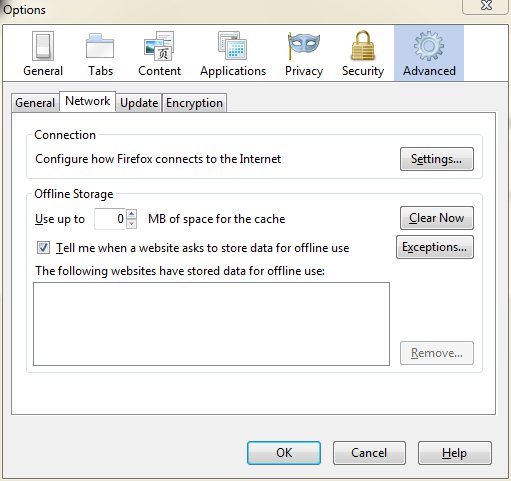
\includegraphics{i2p_1.jpg}
\caption{I2P}
\end{figure}

In the Connection Settings window, click the circle next to Manual proxy
configuration, then enter 127.0.0.1, port 4444 in the HTTP Proxy field.
Enter 127.0.0.1, port 4445 in the SSL Proxy field. Be sure to enter
localhost and 127.0.0.1 into the ``No Proxy for'' box.

\begin{figure}[htbp]
\centering
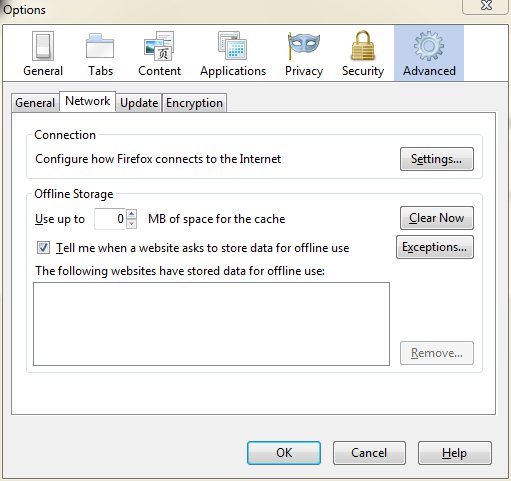
\includegraphics{i2p_1.jpg}
\caption{I2P}
\end{figure}

For more information and proxy settings for other browsers check
\href{http://www.i2p2.de/htproxyports.htm}{http://www.i2p2.de/htproxyports.htm}
